\documentclass{cmn}

\newcommand\vertEq{\rotatebox{90}{=}}

\newlength\cellWidth
\newlength\cellHeight
\setlength\cellWidth{14mm}
\setlength\cellHeight{10mm}

\begin{document}
  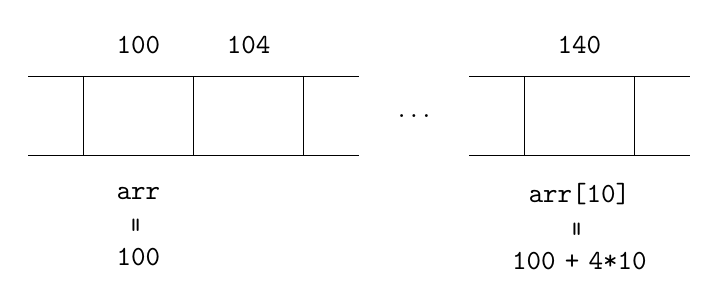
\begin{tikzpicture}
    % borders
    \draw (0,0) -- ++(3*\cellWidth,0);
    \draw (4*\cellWidth,0) -- ++(2*\cellWidth,0);
    \draw (0,-\cellHeight) -- ++(3*\cellWidth,0);
    \draw (4*\cellWidth,-\cellHeight) -- ++(2*\cellWidth,0);

    % cell dividing borders
    \foreach \x in {0,1,2,4,5} {
      \pgfmathsetmacro\nx{\x+0.5}
      \draw (\nx*\cellWidth,0) -- ++(0,-\cellHeight);
    }

    % cell top labels
    \foreach \x/\txt in {1/100,2/104,5/140} {
      \node at (\x*\cellWidth,4mm) {\texttt{\txt}};
    }

    % cell dots
    \node at (3.5*\cellWidth,-\cellHeight/2) {$\dots$};

    % cell bottom labels
    \foreach \x/\txt in {1/arr\\ \vertEq\\ 100,5/arr[10]\\ \vertEq\\ 100 + 4*10} {
      \node[text width=22mm,align=center] at (\x*\cellWidth,-\cellHeight-9mm) {\texttt{\txt}};
    }
  \end{tikzpicture}
\end{document}
